\documentclass[10pt,leqno]{article}
\usepackage[margin=1in]{geometry}
\usepackage{lscape}
\pagenumbering{arabic}
\usepackage{booktabs}
\usepackage{threeparttable}
\usepackage{tabularx}
\usepackage{lscape}
\usepackage{float}
\usepackage{adjustbox}
%\usepackage[landscape]{geometry}
\usepackage{lscape}
\usepackage{amsmath}
\usepackage[T1]{fontenc}
\usepackage[utf8]{inputenc}
\usepackage{pdfpages}
\usepackage{amsmath}
\usepackage{amsfonts}
\usepackage{titlesec}
\usepackage{subfiles}
\titlelabel{\thetitle.\quad}
\usepackage{amssymb}% http://ctan.org/pkg/amssymb
\usepackage{pifont}% http://ctan.org/pkg/pifont
\newcommand{\cmark}{\ding{51}}%
\newcommand{\xmark}{\ding{55}}%
\usepackage{comment}
\usepackage{setspace}
\usepackage{lastpage}
\usepackage{palatino}
\usepackage{float}
\usepackage{titling} 
\usepackage{multirow}
\usepackage{lscape}
\usepackage{amsmath}
\usepackage{amssymb}
\usepackage{subcaption}
\title{Task 5\\
Applied Empirical Economics I}
\author{Fadhil Nadhif Muharam}
\date{\today}

\begin{document}

\maketitle

\section{Cross-fit Partial Out}

\begin{table}[H]
\centering
\caption{Estimated effect of cash bonus on log unemployment duration}
{
\def\sym#1{\ifmmode^{#1}\else\(^{#1}\)\fi}
\begin{tabular}{l*{3}{c}}
\hline\hline
                    &\multicolumn{1}{c}{(1)}         &\multicolumn{1}{c}{(2)}         &\multicolumn{1}{c}{(3)}         \\
                   &\multicolumn{1}{c}{Plugin-formula}         &\multicolumn{1}{c}{Plugin-Always Select}         &\multicolumn{1}{c}{Cross Validation}         \\

\hline
Treatment           &     -0.0814\sym{*}  &     -0.0689         &     -0.0823\sym{*}  \\
                    &    (0.0355)         &    (0.0352)         &    (0.0357)         \\
\hline
Observations        &        5099         &        5099         &        5099         \\
\hline\hline
\multicolumn{4}{l}{\footnotesize Cluster standard errors at location level in parentheses}\\
\multicolumn{4}{l}{\footnotesize \sym{*} \(p<0.05\), \sym{**} \(p<0.01\), \sym{***} \(p<0.001\)}\\
\end{tabular}
}

\end{table}

From Table 1 above and comparing the results with Table 1 in Chernozhukov et al. (2018), the results for the plugin formula and cross-validation on the effect of the treatment on log unemployment are similar. Note that instead of resampling 15 times, I did it 10 times due to my computer limitations. 
\\
\\
\textbf{Plugin-formula}. Using the plugin-formula, the coefficient in Table 1 is statistically significant at 5\% level. The specific number of covariates selected in each fold and resample is shown in Table 2. On average this method selects 5 covariates for log duration of unemployment and 3 for treatment. In Table 3, it is shown the covariates selected for fold 3 and resample 5.
\\
\\
\textbf{Plugin-formula with always select}. Using the plugin-formula with always select, the coefficient in Table 1 is not statistically significant. The specific number of covariates selected in each fold and resample is shown in Table 4. On average this method selects 2 additional covariates on top of the always selected covariates for both log duration of unemployment and treatment. In Table 5, it is shown the covariates selected for fold 3 and resample 5.
\\
\\
\textbf{Cross-validation}. Using the cross-validation, the coefficient in Table 1 is statistically significant at 5\% level. The specific number of covariates selected in each fold and resample is shown in Table 6. On average this method selects 97 covariates for log duration of unemployment and 16 for treatment. In Table 7, it is shown the covariates selected for fold 3 and resample 5.
\\
\pagebreak
\subsection{Plugin Formula}
\begin{table}[H]
  \centering
  \caption{Number of selected variables in each fold and resample (plugin-formula)}
  \label{tab:1}
  \resizebox{0.35\textwidth}{!}{
   \begin{tabular}{l*{4}{c}}
\hline\hline
                    &    resample&       xfold&      lambda&     nonzero\\
\hline
Log duration of unemployment&           1&           1&    .0750276&           6\\
Log duration of unemployment&           1&           2&    .0750779&           4\\
Log duration of unemployment&           1&           3&    .0750697&           4\\
Log duration of unemployment&           1&           4&    .0750861&           4\\
Log duration of unemployment&           1&           5&     .075045&           3\\
Log duration of unemployment&           2&           1&    .0750851&           4\\
Log duration of unemployment&           2&           2&    .0750367&           3\\
Log duration of unemployment&           2&           3&    .0750656&           4\\
Log duration of unemployment&           2&           4&     .075082&           5\\
Log duration of unemployment&           2&           5&    .0750491&           4\\
Log duration of unemployment&           3&           1&    .0750606&           5\\
Log duration of unemployment&           3&           2&    .0750574&           4\\
Log duration of unemployment&           3&           3&     .075082&           5\\
Log duration of unemployment&           3&           4&    .0750861&           4\\
Log duration of unemployment&           3&           5&    .0750284&           5\\
Log duration of unemployment&           4&           1&    .0750318&           3\\
Log duration of unemployment&           4&           2&    .0750491&           4\\
Log duration of unemployment&           4&           3&    .0750491&           4\\
Log duration of unemployment&           4&           4&    .0751064&           3\\
Log duration of unemployment&           4&           5&     .075082&           3\\
Log duration of unemployment&           5&           1&    .0750276&           3\\
Log duration of unemployment&           5&           2&    .0750697&           4\\
Log duration of unemployment&           5&           3&    .0750779&           4\\
Log duration of unemployment&           5&           4&    .0750697&           4\\
Log duration of unemployment&           5&           5&    .0750779&           5\\
Log duration of unemployment&           6&           1&    .0750647&           5\\
Log duration of unemployment&           6&           2&    .0750574&           5\\
Log duration of unemployment&           6&           3&    .0750901&           5\\
Log duration of unemployment&           6&           4&    .0750409&           4\\
Log duration of unemployment&           6&           5&    .0750491&           4\\
Log duration of unemployment&           7&           1&    .0750688&           4\\
Log duration of unemployment&           7&           2&    .0750532&           4\\
Log duration of unemployment&           7&           3&    .0750656&           5\\
Log duration of unemployment&           7&           4&    .0750326&           7\\
Log duration of unemployment&           7&           5&     .075082&           3\\
Log duration of unemployment&           8&           1&     .075077&           4\\
Log duration of unemployment&           8&           2&    .0750697&           4\\
Log duration of unemployment&           8&           3&    .0750574&           3\\
Log duration of unemployment&           8&           4&     .075045&           4\\
Log duration of unemployment&           8&           5&    .0750779&           5\\
Log duration of unemployment&           9&           1&    .0750647&           4\\
Log duration of unemployment&           9&           2&    .0750201&           5\\
Log duration of unemployment&           9&           3&    .0750779&           6\\
Log duration of unemployment&           9&           4&    .0750901&           4\\
Log duration of unemployment&           9&           5&    .0750574&           5\\
Log duration of unemployment&          10&           1&    .0750606&           3\\
Log duration of unemployment&          10&           2&    .0750697&           5\\
Log duration of unemployment&          10&           3&    .0750779&           4\\
Log duration of unemployment&          10&           4&    .0750409&           3\\
Log duration of unemployment&          10&           5&    .0750738&           5\\
Treatment           &           1&           1&    .0750276&           2\\
Treatment           &           1&           2&    .0750779&           4\\
Treatment           &           1&           3&    .0750697&           2\\
Treatment           &           1&           4&    .0750861&           3\\
Treatment           &           1&           5&     .075045&           0\\
Treatment           &           2&           1&    .0750851&           2\\
Treatment           &           2&           2&    .0750367&           1\\
Treatment           &           2&           3&    .0750656&          12\\
Treatment           &           2&           4&     .075082&           1\\
Treatment           &           2&           5&    .0750491&           0\\
Treatment           &           3&           1&    .0750606&           4\\
Treatment           &           3&           2&    .0750574&           2\\
Treatment           &           3&           3&     .075082&           1\\
Treatment           &           3&           4&    .0750861&          10\\
Treatment           &           3&           5&    .0750284&           3\\
Treatment           &           4&           1&    .0750318&           2\\
Treatment           &           4&           2&    .0750491&           2\\
Treatment           &           4&           3&    .0750491&           1\\
Treatment           &           4&           4&    .0751064&           3\\
Treatment           &           4&           5&     .075082&           3\\
Treatment           &           5&           1&    .0750276&           1\\
Treatment           &           5&           2&    .0750697&           2\\
Treatment           &           5&           3&    .0750779&           6\\
Treatment           &           5&           4&    .0750697&           1\\
Treatment           &           5&           5&    .0750779&           2\\
Treatment           &           6&           1&    .0750647&           2\\
Treatment           &           6&           2&    .0750574&           2\\
Treatment           &           6&           3&    .0750901&          10\\
Treatment           &           6&           4&    .0750409&           0\\
Treatment           &           6&           5&    .0750491&           2\\
Treatment           &           7&           1&    .0750688&           0\\
Treatment           &           7&           2&    .0750532&           1\\
Treatment           &           7&           3&    .0750656&           4\\
Treatment           &           7&           4&    .0750326&           1\\
Treatment           &           7&           5&     .075082&           1\\
Treatment           &           8&           1&     .075077&           1\\
Treatment           &           8&           2&    .0750697&           4\\
Treatment           &           8&           3&    .0750574&           1\\
Treatment           &           8&           4&     .075045&           2\\
Treatment           &           8&           5&    .0750779&           2\\
Treatment           &           9&           1&    .0750647&           2\\
Treatment           &           9&           2&    .0750201&           3\\
Treatment           &           9&           3&    .0750779&           2\\
Treatment           &           9&           4&    .0750901&           0\\
Treatment           &           9&           5&    .0750574&           3\\
Treatment           &          10&           1&    .0750606&           1\\
Treatment           &          10&           2&    .0750697&           0\\
Treatment           &          10&           3&    .0750779&           9\\
Treatment           &          10&           4&    .0750409&           3\\
Treatment           &          10&           5&    .0750738&           2\\
\hline\hline
\end{tabular}
 }
\end{table}%

\begin{table}[H]
  \centering
  \caption{Selected variables (fold 3, resample 5) - (plugin-formula)}
  \label{tab:1}
  \resizebox{0.5\textwidth}{!}{
   \begin{tabular}{l*{2}{c}}
\hline\hline
                    &loginuidur\_3\_5&treatment\_3\_5\\
\hline
Recall experiment   &          .x&            \\
Quarter 6 X Quarter 6&          .x&            \\
Quarter 6 X Quarter 2&          .x&            \\
Type of occupation X Age LT 35&          .x&            \\
Location 10677 X Other race&            &          .x\\
Location 10691 X Other race&            &          .x\\
Location 10698 X Other race&            &          .x\\
Location 10726 X Other race&            &          .x\\
Location 10754 X Other race&            &          .x\\
Location 10866 X Hispanic&            &          .x\\
Constant            &          .x&          .x\\
\hline\hline
\end{tabular}
 }
\end{table}%

\pagebreak
\subsection{Plugin Formula with Always Select}
\begin{table}[H]
  \centering
  \caption{Number of selected variables in each fold and resample (plugin-formula, always select)}
  \label{tab:1}
  \resizebox{0.35\textwidth}{!}{
   \begin{tabular}{l*{4}{c}}
\hline\hline
                    &    resample&       xfold&      lambda&     nonzero\\
\hline
Log duration of unemployment&           1&           1&    .0748495&          88\\
Log duration of unemployment&           1&           2&    .0748279&          87\\
Log duration of unemployment&           1&           3&    .0748629&          86\\
Log duration of unemployment&           1&           4&    .0748235&          88\\
Log duration of unemployment&           1&           5&    .0748629&          86\\
Log duration of unemployment&           2&           1&    .0748798&          86\\
Log duration of unemployment&           2&           2&    .0748454&          87\\
Log duration of unemployment&           2&           3&    .0748802&          87\\
Log duration of unemployment&           2&           4&    .0748454&          88\\
Log duration of unemployment&           2&           5&    .0748542&          88\\
Log duration of unemployment&           3&           1&    .0748495&          86\\
Log duration of unemployment&           3&           2&    .0748367&          87\\
Log duration of unemployment&           3&           3&    .0748715&          87\\
Log duration of unemployment&           3&           4&    .0748715&          86\\
Log duration of unemployment&           3&           5&    .0748672&          88\\
Log duration of unemployment&           4&           1&    .0748276&          87\\
Log duration of unemployment&           4&           2&    .0748585&          86\\
Log duration of unemployment&           4&           3&    .0748411&          88\\
Log duration of unemployment&           4&           4&    .0748498&          87\\
Log duration of unemployment&           4&           5&    .0748759&          89\\
Log duration of unemployment&           5&           1&    .0748798&          88\\
Log duration of unemployment&           5&           2&    .0748672&          87\\
Log duration of unemployment&           5&           3&    .0748931&          86\\
Log duration of unemployment&           5&           4&    .0748367&          87\\
Log duration of unemployment&           5&           5&    .0748672&          87\\
Log duration of unemployment&           6&           1&    .0748755&          86\\
Log duration of unemployment&           6&           2&    .0748585&          87\\
Log duration of unemployment&           6&           3&    .0748192&          87\\
Log duration of unemployment&           6&           4&    .0748888&          87\\
Log duration of unemployment&           6&           5&    .0748715&          87\\
Log duration of unemployment&           7&           1&    .0749055&          87\\
Log duration of unemployment&           7&           2&    .0748585&          88\\
Log duration of unemployment&           7&           3&    .0748367&          87\\
Log duration of unemployment&           7&           4&    .0748715&          87\\
Log duration of unemployment&           7&           5&    .0748802&          86\\
Log duration of unemployment&           8&           1&    .0748451&          86\\
Log duration of unemployment&           8&           2&    .0748802&          88\\
Log duration of unemployment&           8&           3&    .0748629&          88\\
Log duration of unemployment&           8&           4&    .0748759&          87\\
Log duration of unemployment&           8&           5&    .0748759&          87\\
Log duration of unemployment&           9&           1&    .0748841&          89\\
Log duration of unemployment&           9&           2&    .0748931&          87\\
Log duration of unemployment&           9&           3&    .0748585&          86\\
Log duration of unemployment&           9&           4&    .0748974&          87\\
Log duration of unemployment&           9&           5&    .0747971&          86\\
Log duration of unemployment&          10&           1&    .0748364&          87\\
Log duration of unemployment&          10&           2&    .0748367&          88\\
Log duration of unemployment&          10&           3&     .074906&          86\\
Log duration of unemployment&          10&           4&    .0748498&          87\\
Log duration of unemployment&          10&           5&    .0748498&          88\\
Treatment           &           1&           1&    .0748407&          87\\
Treatment           &           1&           2&    .0749189&          87\\
Treatment           &           1&           3&    .0748715&          91\\
Treatment           &           1&           4&    .0748802&          86\\
Treatment           &           1&           5&    .0748672&          88\\
Treatment           &           2&           1&    .0748495&          87\\
Treatment           &           2&           2&    .0748454&          88\\
Treatment           &           2&           3&    .0748802&          90\\
Treatment           &           2&           4&    .0748454&          87\\
Treatment           &           2&           5&    .0748888&          86\\
Treatment           &           3&           1&    .0748581&          86\\
Treatment           &           3&           2&    .0748323&          88\\
Treatment           &           3&           3&    .0748974&          87\\
Treatment           &           3&           4&    .0748672&          86\\
Treatment           &           3&           5&    .0748542&          87\\
Treatment           &           4&           1&    .0748407&          88\\
Treatment           &           4&           2&    .0748802&          86\\
Treatment           &           4&           3&    .0748367&          90\\
Treatment           &           4&           4&    .0748672&          89\\
Treatment           &           4&           5&    .0748585&          87\\
Treatment           &           5&           1&    .0748581&          88\\
Treatment           &           5&           2&    .0748411&          86\\
Treatment           &           5&           3&    .0748802&          87\\
Treatment           &           5&           4&    .0748148&          88\\
Treatment           &           5&           5&    .0749017&          92\\
Treatment           &           6&           1&    .0748276&          88\\
Treatment           &           6&           2&    .0748323&          86\\
Treatment           &           6&           3&    .0747838&          88\\
Treatment           &           6&           4&    .0748888&          87\\
Treatment           &           6&           5&    .0748845&          86\\
Treatment           &           7&           1&    .0748711&          88\\
Treatment           &           7&           2&    .0748542&          88\\
Treatment           &           7&           3&    .0748454&          86\\
Treatment           &           7&           4&    .0748672&          88\\
Treatment           &           7&           5&    .0748715&          87\\
Treatment           &           8&           1&    .0748407&          89\\
Treatment           &           8&           2&    .0748629&          87\\
Treatment           &           8&           3&    .0748585&          86\\
Treatment           &           8&           4&    .0748759&          87\\
Treatment           &           8&           5&    .0748845&          88\\
Treatment           &           9&           1&    .0748711&          86\\
Treatment           &           9&           2&    .0748585&          88\\
Treatment           &           9&           3&    .0748629&          91\\
Treatment           &           9&           4&    .0748411&          86\\
Treatment           &           9&           5&    .0747927&          89\\
Treatment           &          10&           1&    .0748451&          88\\
Treatment           &          10&           2&    .0748498&          86\\
Treatment           &          10&           3&    .0748888&          88\\
Treatment           &          10&           4&    .0748759&          87\\
Treatment           &          10&           5&    .0748367&          87\\
\hline\hline
\end{tabular}
 }
\end{table}%

\begin{table}[H]
  \centering
  \caption{Selected variables (fold 3, resample 5) - (plugin-formula, always select)}
  \label{tab:1}
  \resizebox{0.35\textwidth}{!}{
   \begin{tabular}{l*{2}{c}}
\hline\hline
                    &loginuidur\_3\_5&treatment\_3\_5\\
\hline
Female              &          .x&          .x\\
Black               &          .x&          .x\\
Hispanic            &          .x&          .x\\
Other race          &          .x&          .x\\
Number of dependents&          .x&          .x\\
Quarter 1           &          .x&          .x\\
Quarter 2           &          .x&          .x\\
Quarter 3           &          .x&          .x\\
Quarter 4           &          .x&          .x\\
Quarter 5           &          .x&          .x\\
Quarter 6           &          .x&          .x\\
Recall experiment   &          .x&          .x\\
Age LT 35           &          .x&          .x\\
Age GT 54           &          .x&          .x\\
Durable             &          .x&          .x\\
Non-durable         &          .x&          .x\\
Type of occupation  &          .x&          .x\\
Location 10404      &          .x&          .x\\
Location 10411      &          .x&          .x\\
Location 10418      &          .x&          .x\\
Location 10425      &          .x&          .x\\
Location 10432      &          .x&          .x\\
Location 10439      &          .x&          .x\\
Location 10446      &          .x&          .x\\
Location 10453      &          .x&          .x\\
Location 10460      &          .x&          .x\\
Location 10467      &          .x&          .x\\
Location 10474      &          .x&          .x\\
Location 10481      &          .x&          .x\\
Location 10488      &          .x&          .x\\
Location 10495      &          .o&          .o\\
Location 10502      &          .x&          .x\\
Location 10509      &          .x&          .x\\
Location 10516      &          .x&          .x\\
Location 10523      &          .x&          .x\\
Location 10530      &          .x&          .x\\
Location 10537      &          .x&          .x\\
Location 10544      &          .x&          .x\\
Location 10551      &          .x&          .x\\
Location 10558      &          .x&          .x\\
Location 10565      &          .x&          .x\\
Location 10572      &          .x&          .x\\
Location 10579      &          .x&          .x\\
Location 10586      &          .x&          .x\\
Location 10593      &          .x&          .x\\
Location 10600      &          .x&          .x\\
Location 10607      &          .x&          .x\\
Location 10614      &          .x&          .x\\
Location 10621      &          .x&          .x\\
Location 10628      &          .x&          .x\\
Location 10635      &          .x&          .x\\
Location 10642      &          .x&          .x\\
Location 10649      &          .x&          .x\\
Location 10656      &          .x&          .x\\
Location 10663      &          .x&          .x\\
Location 10670      &          .x&          .x\\
Location 10677      &          .x&          .x\\
Location 10684      &          .x&          .x\\
Location 10691      &          .x&          .x\\
Location 10698      &          .x&          .x\\
Location 10705      &          .x&          .x\\
Location 10712      &          .x&          .x\\
Location 10719      &          .x&          .x\\
Location 10726      &          .x&          .x\\
Location 10733      &          .x&          .x\\
Location 10740      &          .x&          .x\\
Location 10747      &          .x&          .x\\
Location 10754      &          .x&          .x\\
Location 10761      &          .x&          .x\\
Location 10768      &          .x&          .x\\
Location 10775      &          .x&          .x\\
Location 10782      &          .x&          .x\\
Location 10789      &          .x&          .x\\
Location 10796      &          .x&          .x\\
Location 10803      &          .x&          .x\\
Location 10810      &          .x&          .x\\
Location 10817      &          .x&          .x\\
Location 10824      &          .x&          .x\\
Location 10831      &          .x&          .x\\
Location 10838      &          .x&          .x\\
Location 10845      &          .x&          .x\\
Location 10852      &          .x&          .x\\
Location 10859      &          .x&          .x\\
Location 10866      &          .x&          .x\\
Location 10873      &          .x&          .x\\
Location 10880      &          .o&          .o\\
Location 10579 X Hispanic&            &          .x\\
Constant            &          .x&          .x\\
\hline\hline
\end{tabular}
 }
\end{table}%

\pagebreak
\subsection{Cross Validation}

\begin{table}[H]
  \centering
  \caption{Number of selected variables in each fold and resample (cross validation)}
  \label{tab:1}
  \resizebox{0.35\textwidth}{!}{
   \begin{tabular}{l*{4}{c}}
\hline\hline
                    &    resample&       xfold&      lambda&     nonzero\\
\hline
Log duration of unemployment&           1&           1&    .0283441&         109\\
Log duration of unemployment&           1&           2&    .0327521&          70\\
Log duration of unemployment&           1&           3&    .0226128&         171\\
Log duration of unemployment&           1&           4&    .0287722&         111\\
Log duration of unemployment&           1&           5&    .0263297&         118\\
Log duration of unemployment&           2&           1&    .0316371&          89\\
Log duration of unemployment&           2&           2&    .0277433&         118\\
Log duration of unemployment&           2&           3&    .0286468&         109\\
Log duration of unemployment&           2&           4&    .0257292&         145\\
Log duration of unemployment&           2&           5&    .0236923&         155\\
Log duration of unemployment&           3&           1&    .0272044&         127\\
Log duration of unemployment&           3&           2&    .0261429&         121\\
Log duration of unemployment&           3&           3&    .0263251&         132\\
Log duration of unemployment&           3&           4&    .0311569&          93\\
Log duration of unemployment&           3&           5&    .0284377&         117\\
Log duration of unemployment&           4&           1&    .0270826&         122\\
Log duration of unemployment&           4&           2&     .027784&         116\\
Log duration of unemployment&           4&           3&    .0257685&         133\\
Log duration of unemployment&           4&           4&     .023484&         147\\
Log duration of unemployment&           4&           5&    .0297331&         116\\
Log duration of unemployment&           5&           1&    .0247635&         154\\
Log duration of unemployment&           5&           2&    .0281957&         105\\
Log duration of unemployment&           5&           3&    .0299684&          98\\
Log duration of unemployment&           5&           4&    .0257743&         130\\
Log duration of unemployment&           5&           5&    .0291404&         106\\
Log duration of unemployment&           6&           1&    .0253261&         152\\
Log duration of unemployment&           6&           2&    .0344363&          66\\
Log duration of unemployment&           6&           3&    .0243924&         157\\
Log duration of unemployment&           6&           4&     .025424&         132\\
Log duration of unemployment&           6&           5&    .0278583&         110\\
Log duration of unemployment&           7&           1&     .028877&         112\\
Log duration of unemployment&           7&           2&    .0270051&         131\\
Log duration of unemployment&           7&           3&     .026942&         116\\
Log duration of unemployment&           7&           4&     .022819&         165\\
Log duration of unemployment&           7&           5&    .0276191&         125\\
Log duration of unemployment&           8&           1&    .0235992&         159\\
Log duration of unemployment&           8&           2&    .0279658&         121\\
Log duration of unemployment&           8&           3&    .0331935&          86\\
Log duration of unemployment&           8&           4&    .0285506&         110\\
Log duration of unemployment&           8&           5&    .0286732&         106\\
Log duration of unemployment&           9&           1&    .0259998&         132\\
Log duration of unemployment&           9&           2&    .0263981&         113\\
Log duration of unemployment&           9&           3&    .0293495&         110\\
Log duration of unemployment&           9&           4&    .0322205&          88\\
Log duration of unemployment&           9&           5&    .0328922&          84\\
Log duration of unemployment&          10&           1&     .025158&         134\\
Log duration of unemployment&          10&           2&    .0255433&         144\\
Log duration of unemployment&          10&           3&    .0294839&         108\\
Log duration of unemployment&          10&           4&    .0269955&         120\\
Log duration of unemployment&          10&           5&    .0330868&          70\\
Treatment           &           1&           1&    .0219511&           0\\
Treatment           &           1&           2&    .0206463&           0\\
Treatment           &           1&           3&    .0213385&           0\\
Treatment           &           1&           4&    .0233642&           0\\
Treatment           &           1&           5&    .0169931&          17\\
Treatment           &           2&           1&     .023069&           0\\
Treatment           &           2&           2&    .0231805&           0\\
Treatment           &           2&           3&    .0247928&           0\\
Treatment           &           2&           4&    .0155535&          24\\
Treatment           &           2&           5&    .0208933&           0\\
Treatment           &           3&           1&    .0229746&           0\\
Treatment           &           3&           2&    .0236595&           0\\
Treatment           &           3&           3&    .0236595&           0\\
Treatment           &           3&           4&    .0225823&           0\\
Treatment           &           3&           5&    .0172168&          17\\
Treatment           &           4&           1&    .0240035&           0\\
Treatment           &           4&           2&    .0230002&           0\\
Treatment           &           4&           3&    .0217962&           0\\
Treatment           &           4&           4&    .0226121&           3\\
Treatment           &           4&           5&     .019178&           0\\
Treatment           &           5&           1&    .0195481&           7\\
Treatment           &           5&           2&    .0213241&           0\\
Treatment           &           5&           3&    .0216637&           0\\
Treatment           &           5&           4&    .0203774&           0\\
Treatment           &           5&           5&     .020654&           0\\
Treatment           &           6&           1&    .0232836&           0\\
Treatment           &           6&           2&    .0212831&           0\\
Treatment           &           6&           3&    .0217595&           0\\
Treatment           &           6&           4&    .0237697&           0\\
Treatment           &           6&           5&    .0225413&           2\\
Treatment           &           7&           1&     .022144&           0\\
Treatment           &           7&           2&    .0242454&           0\\
Treatment           &           7&           3&    .0192895&           5\\
Treatment           &           7&           4&    .0151575&          29\\
Treatment           &           7&           5&    .0201022&           6\\
Treatment           &           8&           1&    .0226554&           0\\
Treatment           &           8&           2&    .0136933&          39\\
Treatment           &           8&           3&    .0231376&           0\\
Treatment           &           8&           4&    .0252984&           0\\
Treatment           &           8&           5&    .0217093&           0\\
Treatment           &           9&           1&    .0228887&           0\\
Treatment           &           9&           2&    .0230174&           0\\
Treatment           &           9&           3&    .0159123&          26\\
Treatment           &           9&           4&    .0227675&           1\\
Treatment           &           9&           5&    .0247809&           0\\
Treatment           &          10&           1&    .0266914&           0\\
Treatment           &          10&           2&    .0207654&           0\\
Treatment           &          10&           3&    .0212673&           0\\
Treatment           &          10&           4&    .0235174&           0\\
Treatment           &          10&           5&    .0230174&           0\\
\hline\hline
\end{tabular}
 }
\end{table}%

\begin{table}[H]
  \centering
  \caption{Selected variables (fold 3, resample 5) - (cross validation)}
  \label{tab:1}
  \resizebox{0.35\textwidth}{!}{
   \begin{tabular}{l*{2}{c}}
\hline\hline
                    &loginuidur\_3\_5&treatment\_3\_5\\
\hline
Age GT 54           &          .x&            \\
Location 10593      &          .x&            \\
Location 10677      &          .x&            \\
Location 10782      &          .x&            \\
Location 10796      &          .x&            \\
Female X Female     &          .x&            \\
Black X Female      &          .x&            \\
Quarter 3 X Black   &          .x&            \\
Quarter 3 X Hispanic&          .x&            \\
Quarter 4 X Other race&          .x&            \\
Quarter 5 X Black   &          .x&            \\
Quarter 5 X Other race&          .x&            \\
Quarter 5 X Number of dependents&          .x&            \\
Quarter 6 X Quarter 6&          .x&            \\
Quarter 6 X Quarter 2&          .x&            \\
Recall experiment X Recall experiment&          .x&            \\
Recall experiment X Quarter 6&          .x&            \\
Age LT 35 X Age LT 35&          .x&            \\
Age LT 35 X Hispanic&          .x&            \\
Age LT 35 X Other race&          .x&            \\
Age LT 35 X Quarter 3&          .x&            \\
Age LT 35 X Quarter 5&          .x&            \\
Age GT 54 X Female  &          .x&            \\
Age GT 54 X Other race&          .x&            \\
Durable X Female    &          .x&            \\
Durable X Black     &          .x&            \\
Durable X Quarter 6 &          .x&            \\
Non-durable X Hispanic&          .x&            \\
Non-durable X Recall experiment&          .x&            \\
Type of occupation X Type of occupation&          .x&            \\
Type of occupation X Black&          .x&            \\
Type of occupation X Quarter 2&          .x&            \\
Type of occupation X Age LT 35&          .x&            \\
Location 10425 X Female&          .x&            \\
Location 10474 X Durable&          .x&            \\
Location 10488 X Quarter 1&          .x&            \\
Location 10516 X Black&          .x&            \\
Location 10516 X Age GT 54&          .x&            \\
Location 10530 X Female&          .x&            \\
Location 10537 X Black&          .x&            \\
Location 10544 X Hispanic&          .x&            \\
Location 10565 X Type of occupation&          .x&            \\
Location 10593 X Age LT 35&          .x&            \\
Location 10593 X Type of occupation&          .x&            \\
Location 10600 X Age GT 54&          .x&            \\
Location 10614 X Type of occupation&          .x&            \\
Location 10621 X Durable&          .x&            \\
Location 10628 X Age LT 35&          .x&            \\
Location 10628 X Durable&          .x&            \\
Location 10635 X Black&          .x&            \\
Location 10635 X Age GT 54&          .x&            \\
Location 10642 X Non-durable&          .x&            \\
Location 10663 X Black&          .x&            \\
Location 10663 X Hispanic&          .x&            \\
Location 10670 X Recall experiment&          .x&            \\
Location 10677 X Quarter 3&          .x&            \\
Location 10677 X Non-durable&          .x&            \\
Location 10684 X Age GT 54&          .x&            \\
Location 10705 X Black&          .x&            \\
Location 10726 X Durable&          .x&            \\
Location 10733 X Female&          .x&            \\
Location 10740 X Non-durable&          .x&            \\
Location 10761 X Age LT 35&          .x&            \\
Location 10761 X Durable&          .x&            \\
Location 10768 X Hispanic&          .x&            \\
Location 10768 X Quarter 6&          .x&            \\
Location 10768 X Durable&          .x&            \\
Location 10782 X Hispanic&          .x&            \\
Location 10789 X Number of dependents&          .x&            \\
Location 10789 X Recall experiment&          .x&            \\
Location 10789 X Durable&          .x&            \\
Location 10796 X Hispanic&          .x&            \\
Location 10796 X Recall experiment&          .x&            \\
Location 10803 X Durable&          .x&            \\
Location 10810 X Hispanic&          .x&            \\
Location 10810 X Non-durable&          .x&            \\
Location 10824 X Black&          .x&            \\
Location 10824 X Number of dependents&          .x&            \\
Location 10824 X Non-durable&          .x&            \\
Location 10824 X Type of occupation&          .x&            \\
Location 10831 X Black&          .x&            \\
Location 10831 X Durable&          .x&            \\
Location 10831 X Non-durable&          .x&            \\
Location 10831 X Type of occupation&          .x&            \\
Location 10838 X Other race&          .x&            \\
Location 10838 X Number of dependents&          .x&            \\
Location 10838 X Quarter 6&          .x&            \\
Location 10866 X Female&          .x&            \\
Location 10866 X Black&          .x&            \\
Location 10873 X Recall experiment&          .x&            \\
Location 10880 X Age LT 35&          .x&            \\
Dep$^2$ X Quarter 4 &          .x&            \\
Dep$^2$ X Quarter 6 &          .x&            \\
Dep$^2$ X Location 10537&          .x&            \\
Dep$^2$ X Location 10705&          .x&            \\
Dep$^2$ X Location 10754&          .x&            \\
Dep$^2$ X Location 10789&          .x&            \\
Dep$^2$ X Location 10796&          .x&            \\
Constant            &          .x&          .x\\
\hline\hline
\end{tabular}
 }
\end{table}%


\pagebreak
\section{Random Forest}
\subsection{Within-time period prediction}
\begin{figure}  [h!]
\begin{center}
\caption{Best tree}
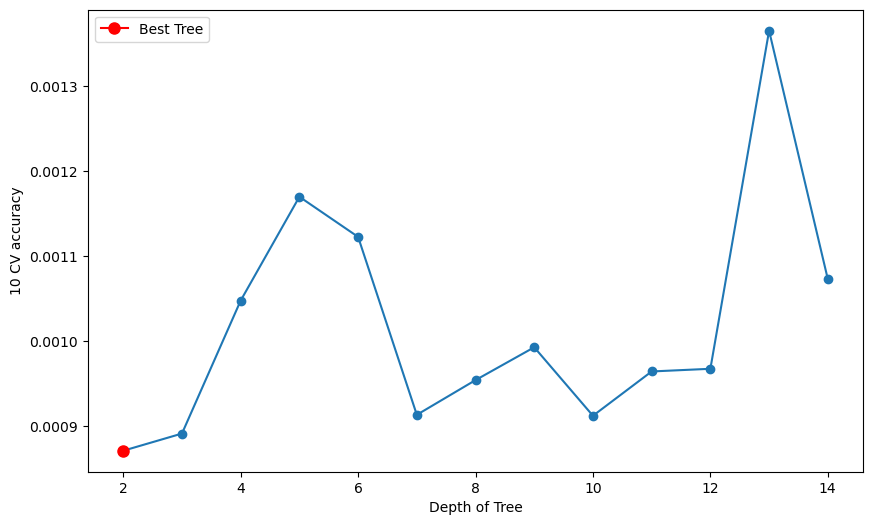
\includegraphics[scale=0.4]{BestTree_RF1.png}
\end{center}
\end{figure}  

\begin{figure}  [h!]
\begin{center}
\caption{Tree plot}
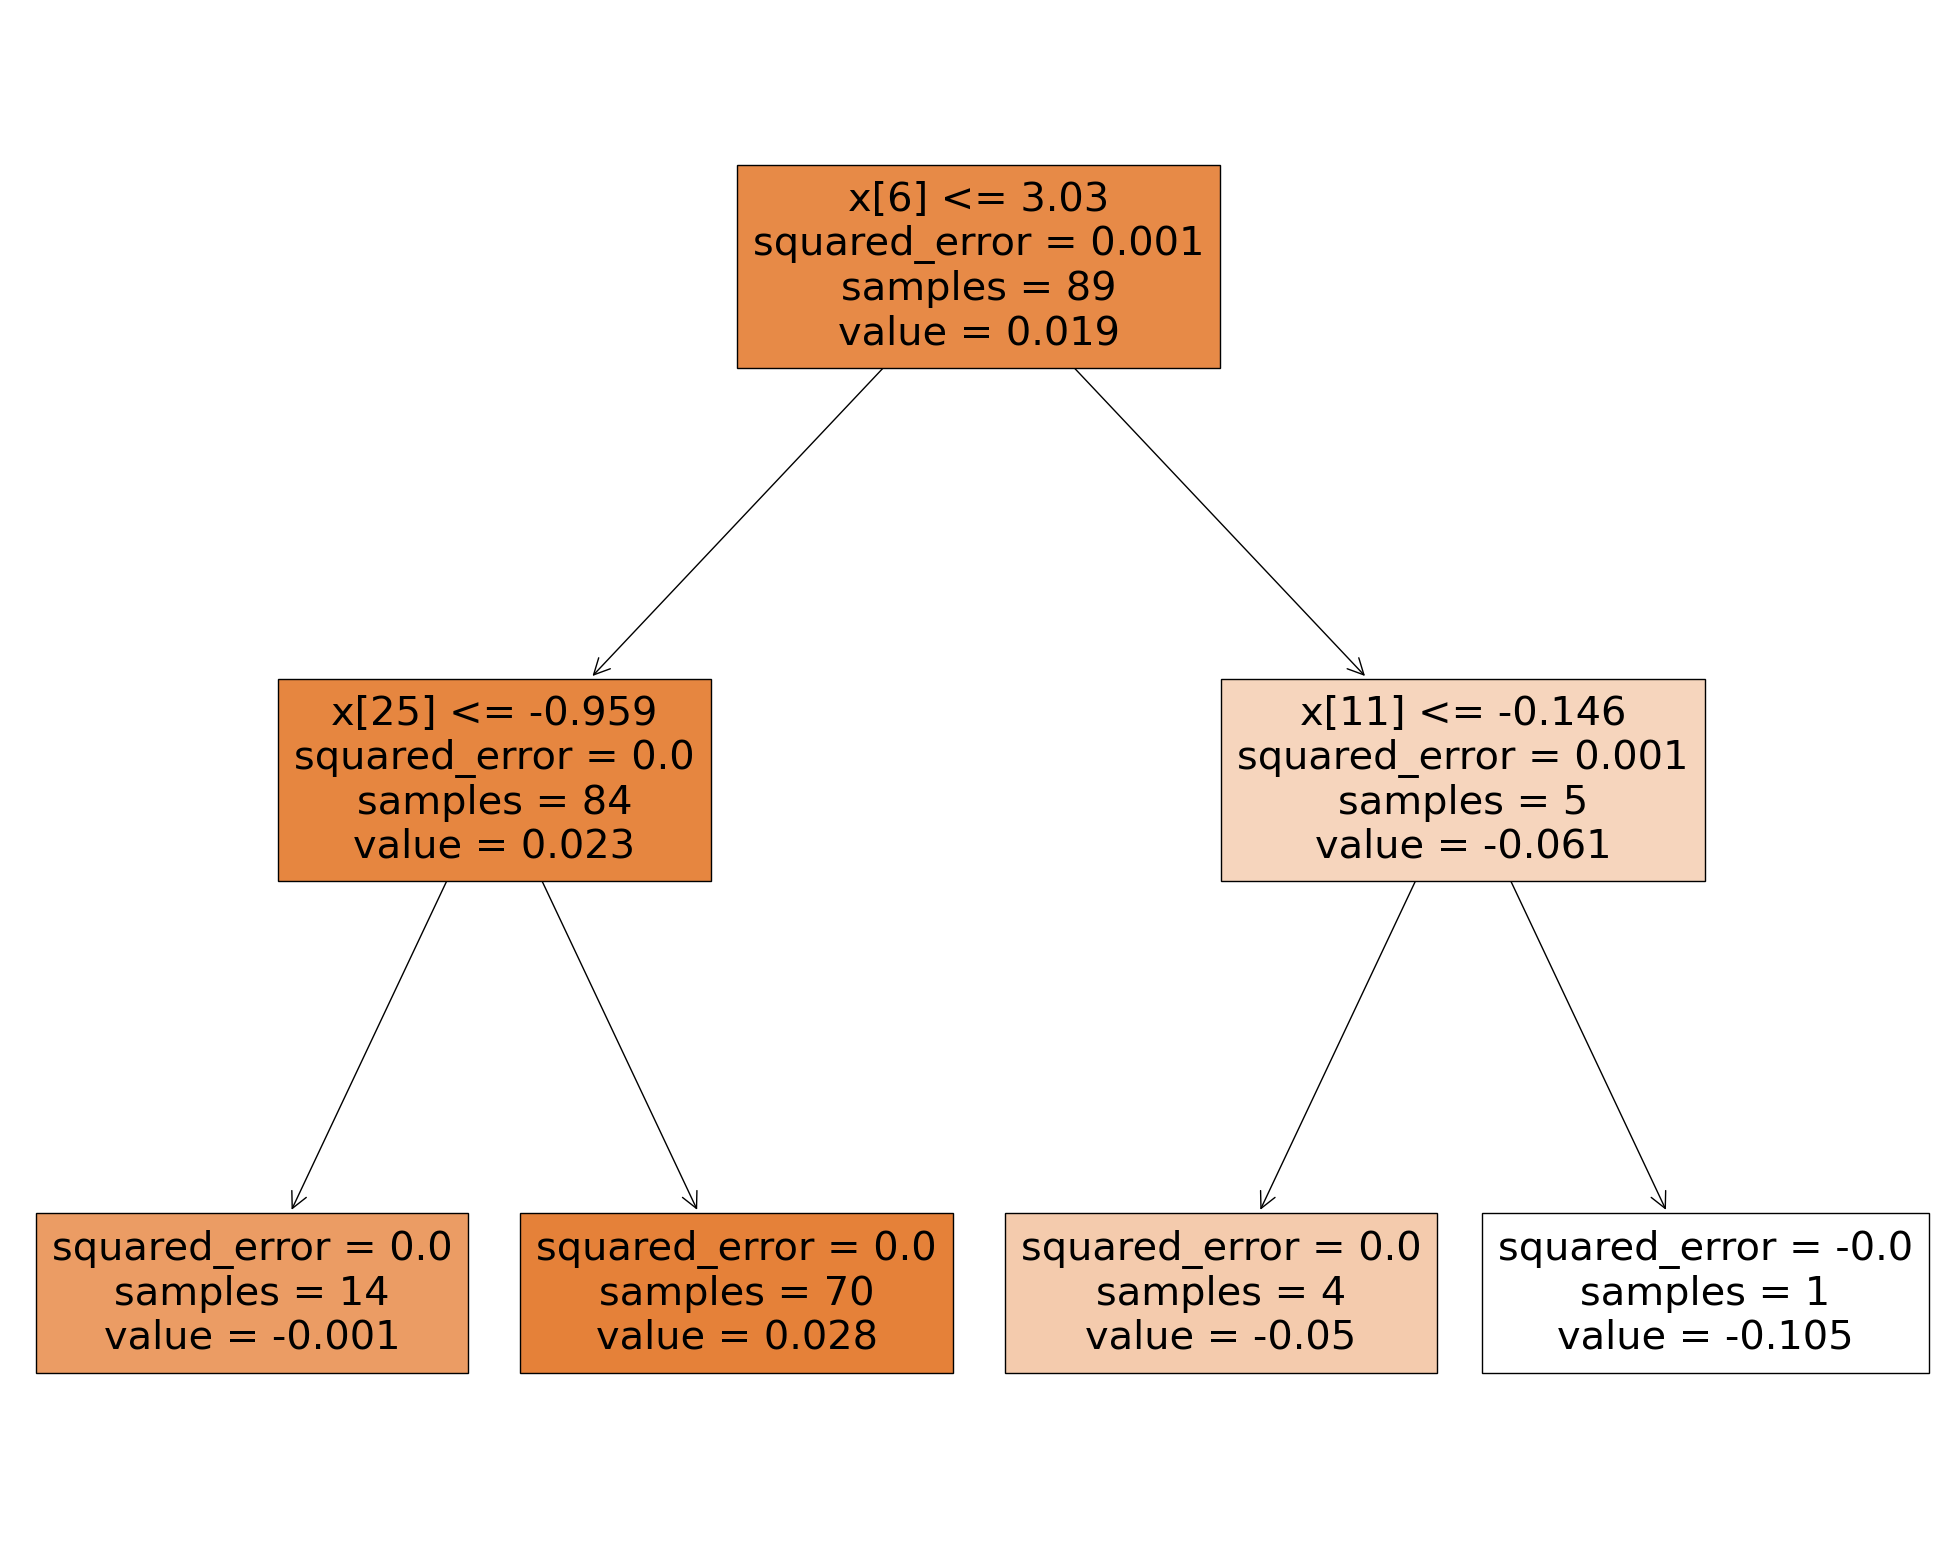
\includegraphics[scale=0.2]{TreePlot_RF1.png}
\end{center}
\end{figure}  

\begin{figure}  [h!]
\begin{center}
\caption{Random forest regressor}
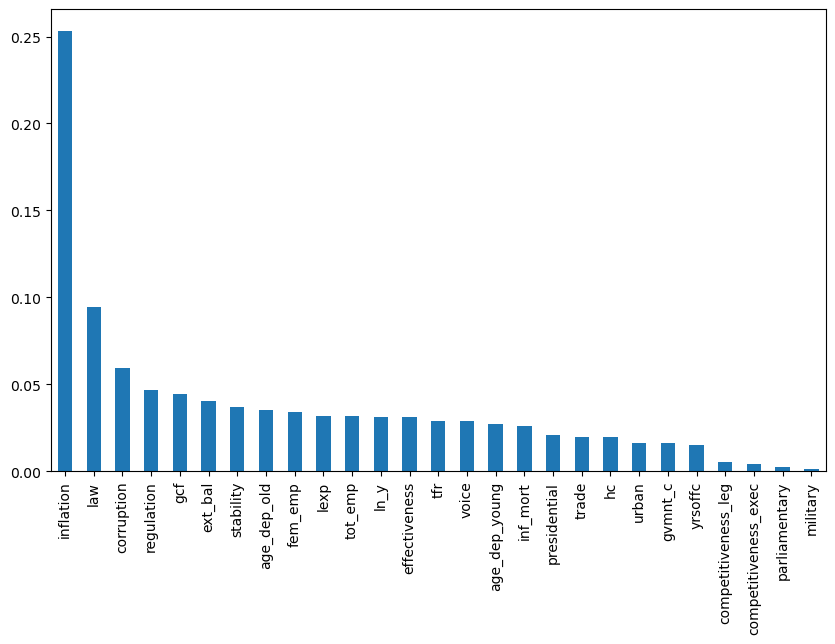
\includegraphics[scale=0.4]{RFRegressor_RF1.png}
\end{center}
\end{figure}  

\pagebreak
\subsection{Out-of-sample prediction}
\begin{figure}  [h!]
\begin{center}
\caption{Best tree}
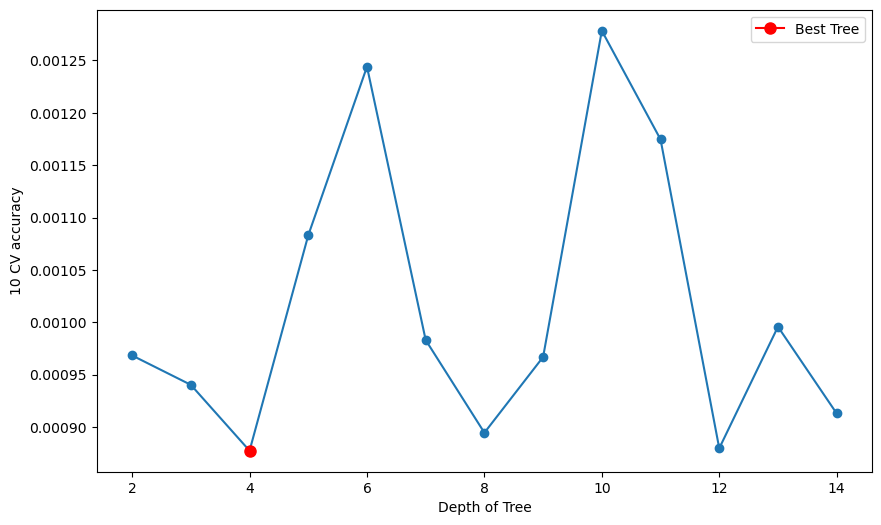
\includegraphics[scale=0.4]{BestTree_RF2.png}
\end{center}
\end{figure}  

\begin{figure}  [h!]
\begin{center}
\caption{Tree plot}
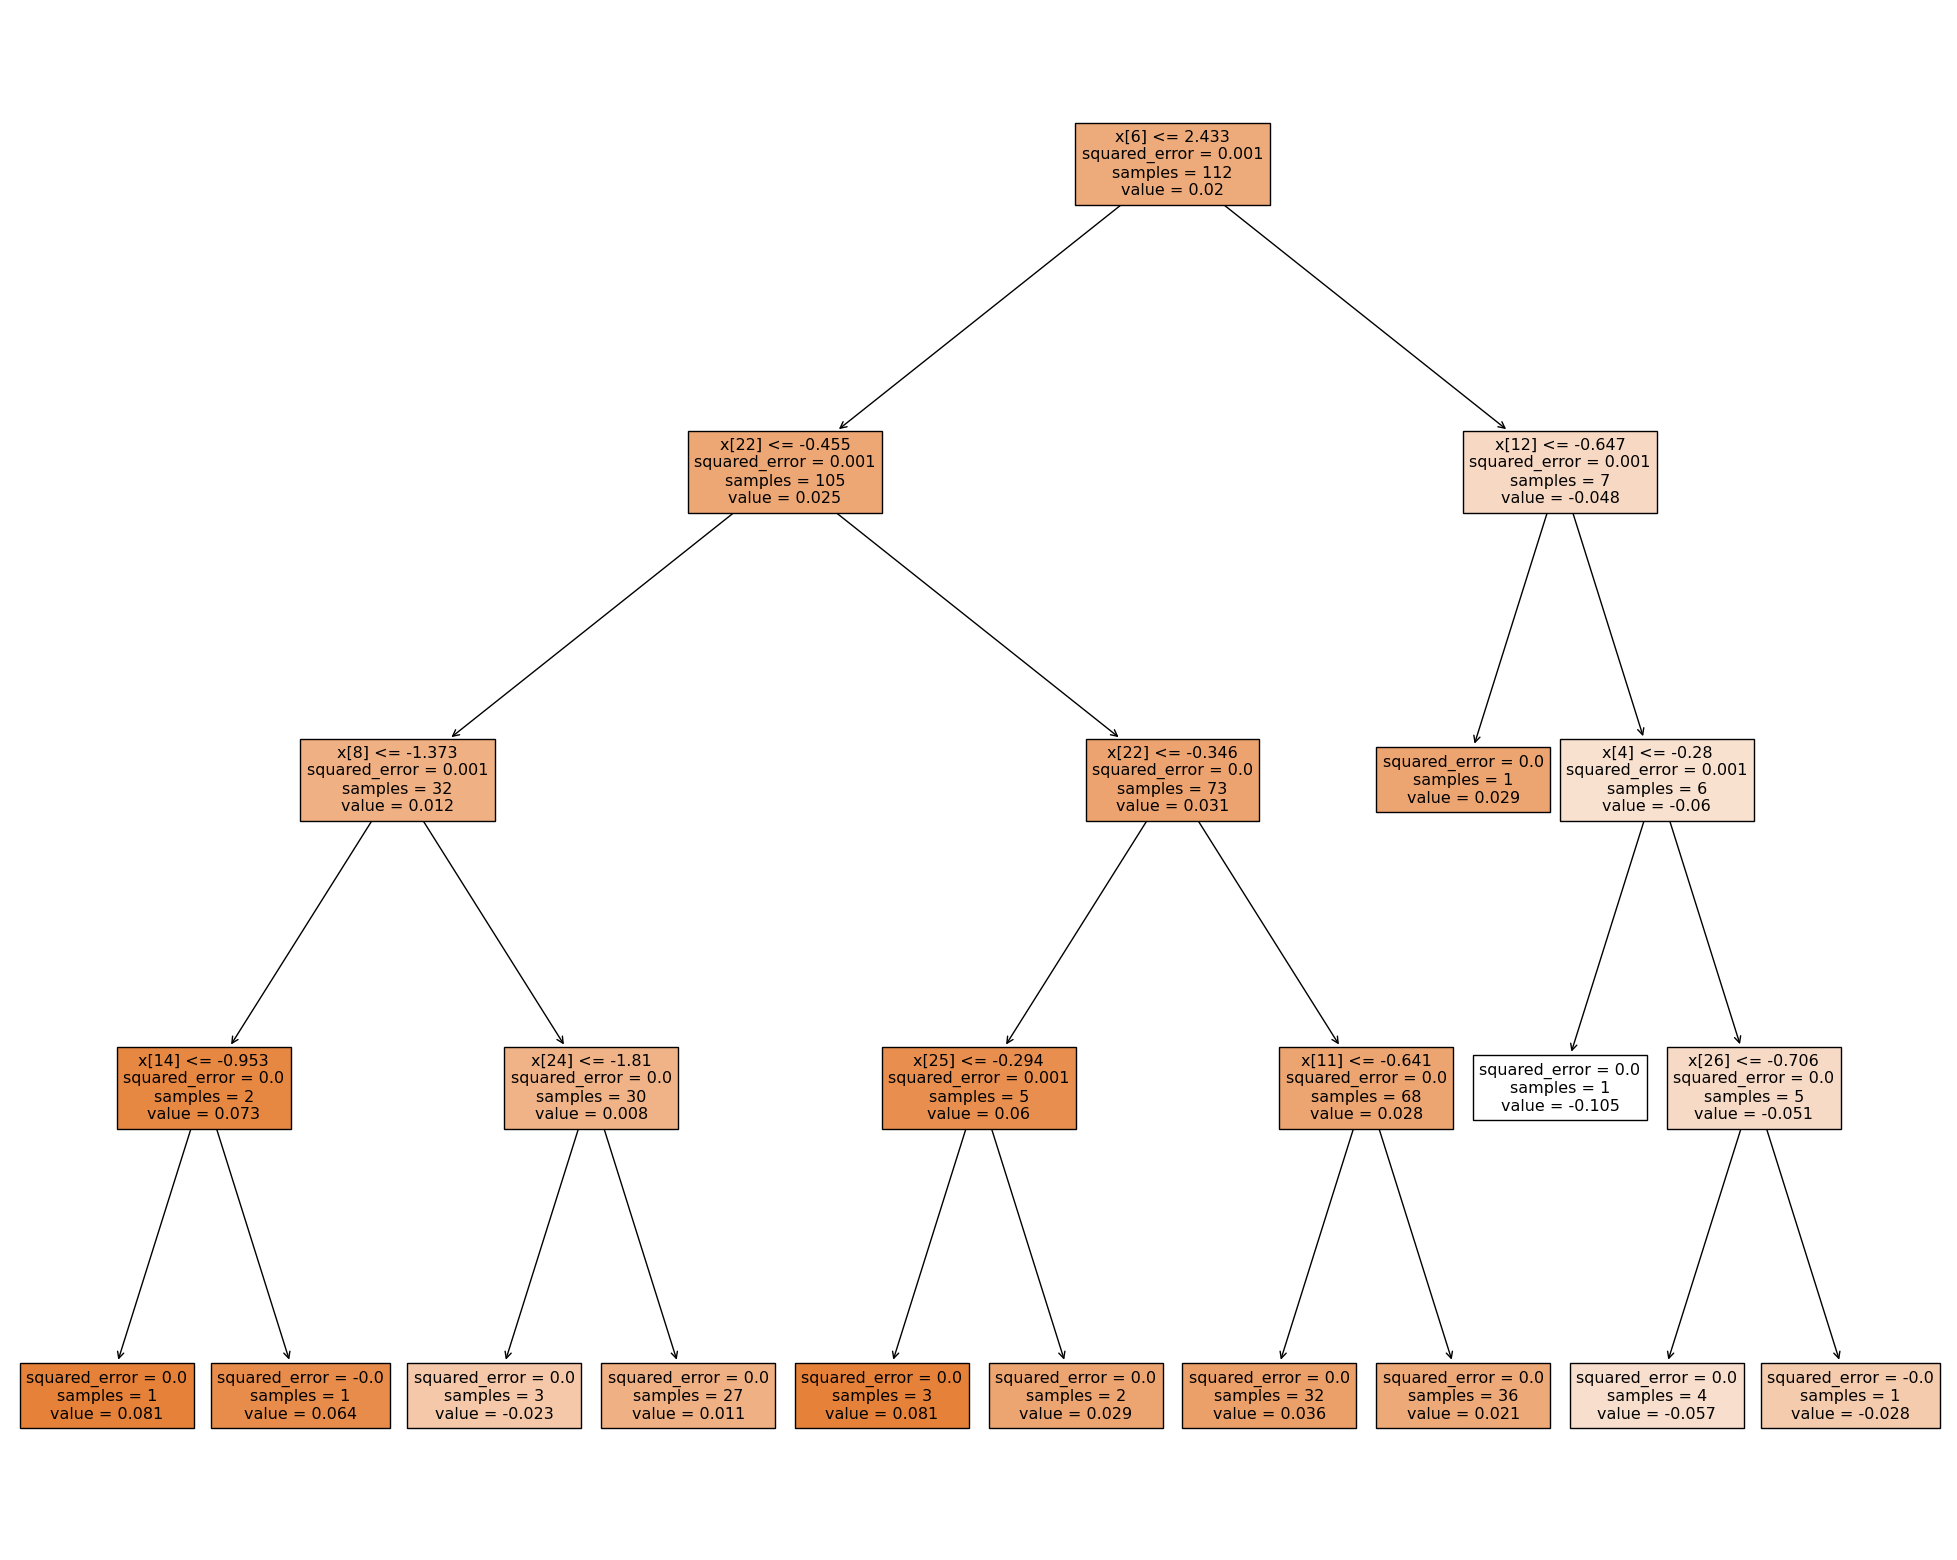
\includegraphics[scale=0.3]{TreePlot_RF2.png}
\end{center}
\end{figure}  

\begin{figure}  [h!]
\begin{center}
\caption{Random forest regressor}
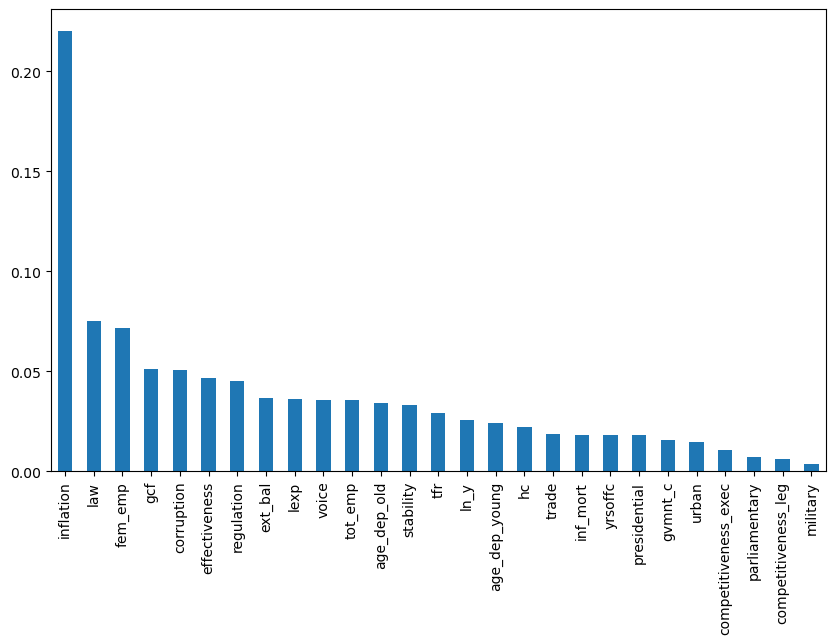
\includegraphics[scale=0.4]{RFRegressor_RF2.png}
\end{center}
\end{figure}  

\pagebreak
\subsection{Testing for changing data generating process}
\begin{figure}  [h!]
\begin{center}
\caption{Best tree}
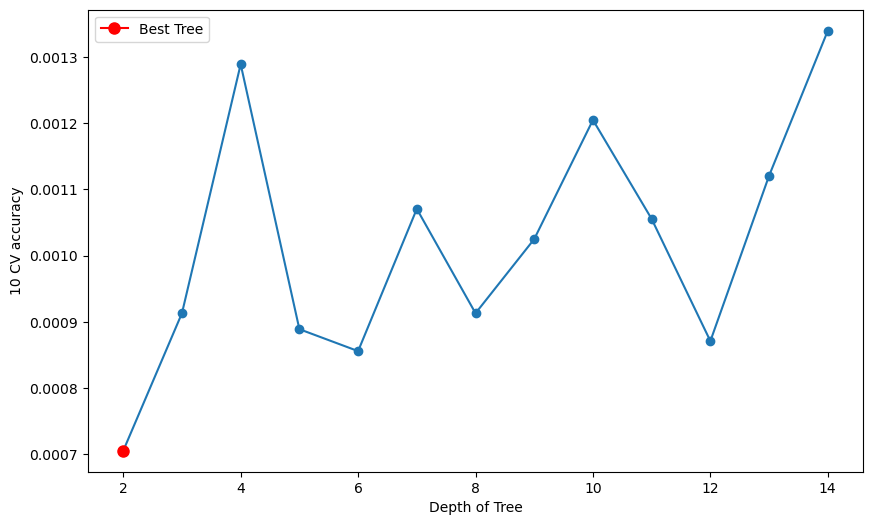
\includegraphics[scale=0.4]{BestTree_RF3.png}
\end{center}
\end{figure}  

\begin{figure}  [h!]
\begin{center}
\caption{Tree plot}
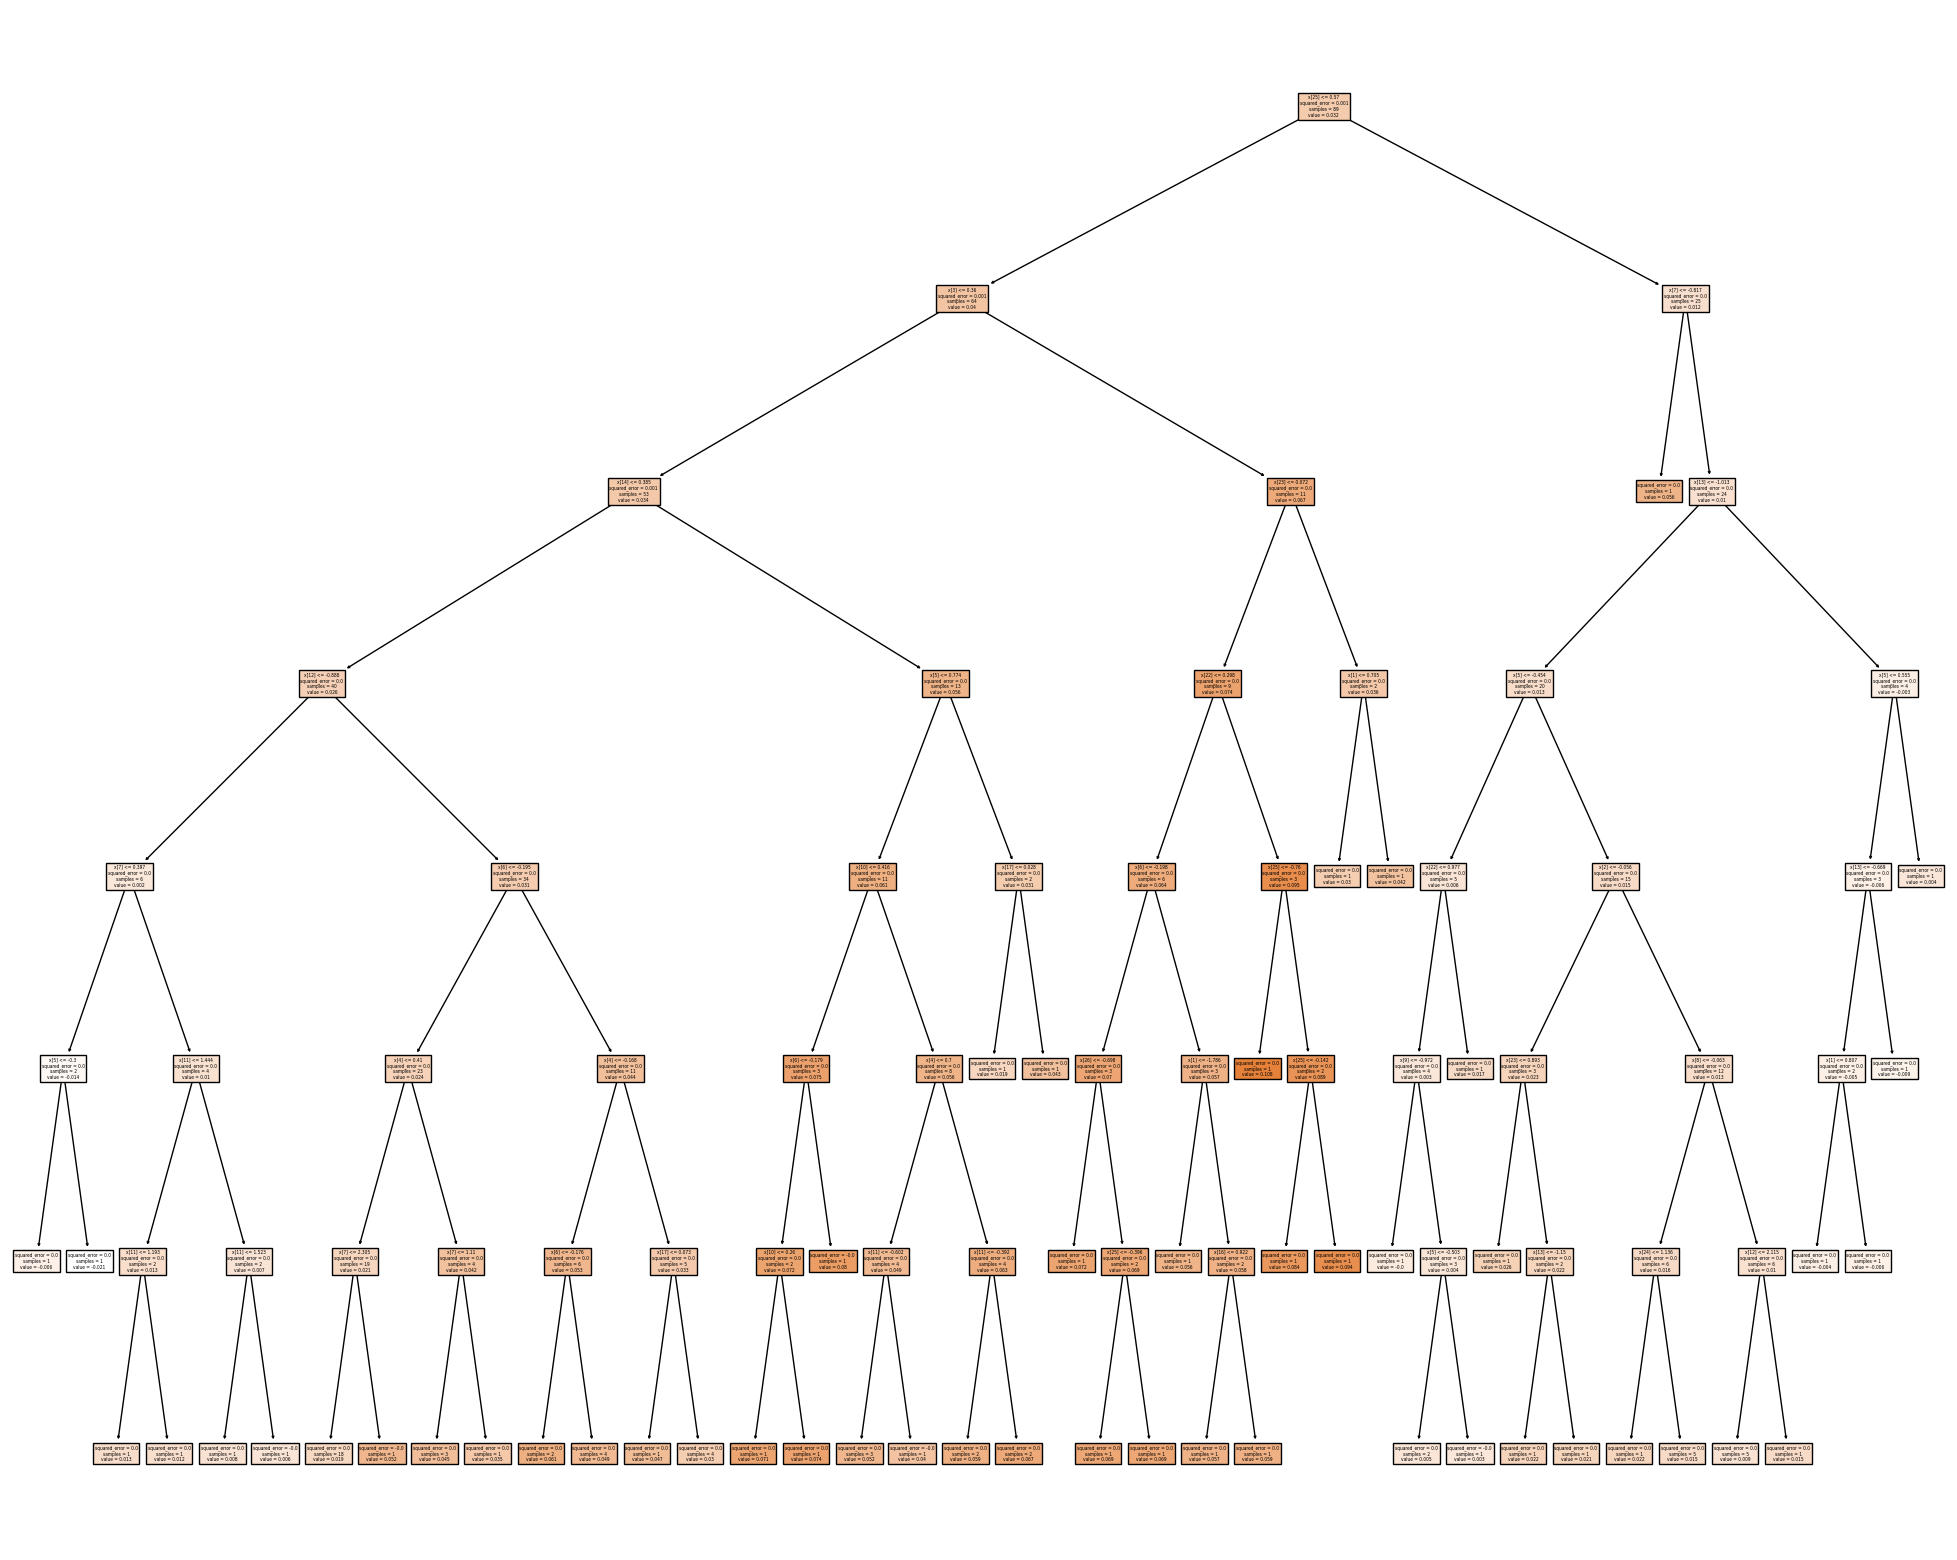
\includegraphics[scale=0.3]{TreePlot_RF3.png}
\end{center}
\end{figure}  

\begin{figure}  [h!]
\begin{center}
\caption{Random forest regressor}
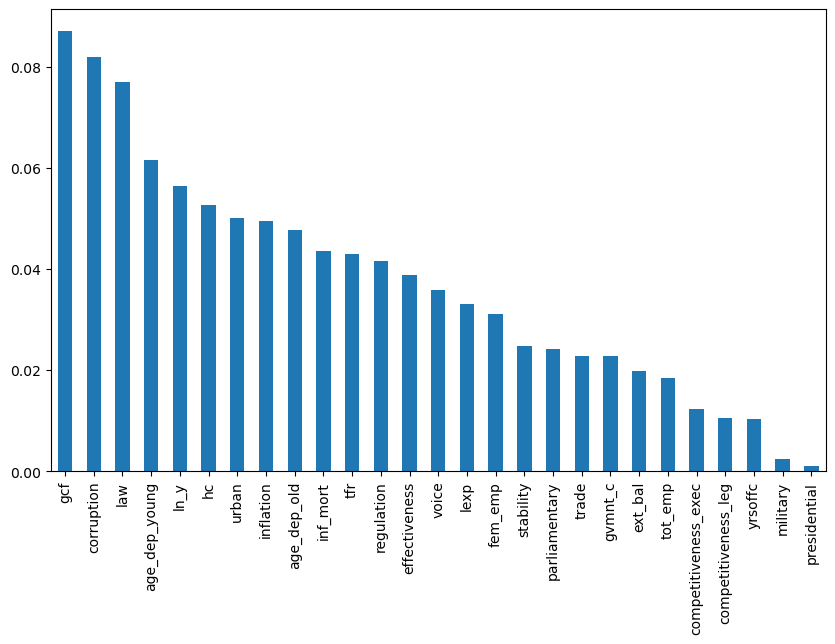
\includegraphics[scale=0.4]{RFRegressor_RF3.png}
\end{center}
\end{figure}  



\end{document}

